%%%%%%%%%%%%%%%%%%%%%%%%%%%%%%%%%%%%%%%%% 
% Masters/Doctoral Thesis 
% LaTeX Template
% Version 2.5 (27/8/17)
%
% This template was downloaded from:
% http://www.LaTeXTemplates.com
%
% Version 2.x major modifications by:
% Vel (vel@latextemplates.com)
%
% This template is based on a template by:
% Steve Gunn (http://users.ecs.soton.ac.uk/srg/softwaretools/document/templates/)
% Sunil Patel (http://www.sunilpatel.co.uk/thesis-template/)
%
% Template license:
% CC BY-NC-SA 3.0 (http://creativecommons.org/licenses/by-nc-sa/3.0/)
%
%%%%%%%%%%%%%%%%%%%%%%%%%%%%%%%%%%%%%%%%%

%----------------------------------------------------------------------------------------
%	PACKAGES AND OTHER DOCUMENT CONFIGURATIONS
%----------------------------------------------------------------------------------------

\documentclass[
11pt, % The default document font size, options: 10pt, 11pt, 12pt
%oneside, % Two side (alternating margins) for binding by default, uncomment to switch to one side
english, % ngerman for German
singlespacing, % Single line spacing, alternatives: onehalfspacing or doublespacing
%draft, % Uncomment to enable draft mode (no pictures, no links, overfull hboxes indicated)
%nolistspacing, % If the document is onehalfspacing or doublespacing, uncomment this to set spacing in lists to single
%liststotoc, % Uncomment to add the list of figures/tables/etc to the table of contents
%toctotoc, % Uncomment to add the main table of contents to the table of contents
%parskip, % Uncomment to add space between paragraphs
%nohyperref, % Uncomment to not load the hyperref package
headsepline, % Uncomment to get a line under the header
%chapterinoneline, % Uncomment to place the chapter title next to the number on one line
%consistentlayout, % Uncomment to change the layout of the declaration, abstract and acknowledgements pages to match the default layout
oneside,
]{MastersDoctoralThesis} % The class file specifying the document structure

\usepackage[utf8]{inputenc} % Required for inputting international characters
\usepackage[T1]{fontenc} % Output font encoding for international characters

\usepackage{mathpazo} % Use the Palatino font by default

%\usepackage[backend=bibtex,style=authoryear,natbib=true]{biblatex} % Use the bibtex backend with the authoryear citation style (which resembles APA)

% does not work with tex live 2009
%\addbibresource{master} % The filename of the bibliography
\usepackage{natbib}

\usepackage[autostyle=true]{csquotes} % Required to generate language-dependent quotes in the bibliography
\usepackage{tabu}
\usepackage{float}
\usepackage{graphicx}
\usepackage{bmpsize}

%----------------------------------------------------------------------------------------
%	MARGIN SETTINGS
%----------------------------------------------------------------------------------------

\geometry{
	paper=a4paper, % Change to letterpaper for US letter
	inner=2.5cm, % Inner margin
	outer=3.8cm, % Outer margin
	bindingoffset=.5cm, % Binding offset
	top=1.5cm, % Top margin
	bottom=1.5cm, % Bottom margin
	%showframe, % Uncomment to show how the type block is set on the page
}


%----------------------------------------------------------------------------------------
%	THESIS INFORMATION
%----------------------------------------------------------------------------------------

\thesistitle{Evaluating phylogenetic methods for quantifying risks and opportunities presented by forks in open source software} % Your thesis title, this is used in the title and abstract, print it elsewhere with \ttitle
\supervisor{Dr. Doug \textsc{Leith}} % Your supervisor's name, this is used in the title page, print it elsewhere with \supname
\degree{Master of Science in Computing (Software Engineering)} % Your degree name, this is used in the title page and abstract, print it elsewhere with \degreename
\author{Alvaro \textsc{Ortiz Troncoso}} % Your name, this is used in the title page and abstract, print it elsewhere with \authorname

\university{\href{http://www.open.ac.uk}{Open University UK}} % Your university's name and URL, this is used in the title page and abstract, print it elsewhere with \univname

%----------------------------------------------------------------------------------------
%	BEGIN CONTENT
%----------------------------------------------------------------------------------------

\AtBeginDocument{
\hypersetup{pdftitle=\ttitle} % Set the PDF's title to your title
\hypersetup{pdfauthor=\authorname} % Set the PDF's author to your name
}
\begin{document}

%\frontmatter % Use roman page numbering style (i, ii, iii, iv...) for the pre-content pages

\pagestyle{empty} % suppress page numbers in the extended abstract

%----------------------------------------------------------------------------------------

\begin{center}

{\scshape \univname\par}\vspace{1.5cm} % University name
\textsc{\Large Extended Abstract}\\[0.5cm] % Thesis type

{\bfseries \ttitle\par}\vspace{0.4cm} % Thesis title

\bigskip

\begin{minipage}[t]{0.4\textwidth}
\begin{flushleft} \large
\emph{Author:}\\
{\authorname} % Author name - remove the \href bracket to remove the link
\end{flushleft}
\end{minipage}
\begin{minipage}[t]{0.4\textwidth}
\begin{flushright} \large
\emph{Supervisor:} \\
{\supname} % Supervisor name - remove the \href bracket to remove the link  
\end{flushright}
\end{minipage}\\[3cm]
 
\end{center}

%----------------------------------------------------------------------------------------

\section*{Motivation and research aim}
The nature of software makes software engineering a different endeavour than other forms of engineering. The artefacts produced during software development can be copied and distributed at almost no cost, challenging traditional business models based on the distribution of physical products and strong intellectual property protection \citep{Kogut2001a}. Besides intellectual property challenges, software development also questions the idea of a development lifecycle resulting in a stable and long-lived product. Software is required to evolve, even after it has been released for production \citep{Lehman1980a}. Software evolution is driven by the changing expectations of its users, a dynamic hardware and software ecosystem and an innovative business environment.

Open source software development is a development paradigm that purports to increase the value of software by embracing these difficulties. Instead of applying strong intellectual property protection to create an economy of scarcity, open source licenses guarantee the free flow of ideas. Furthermore, open source development embraces constantly changing requirements by blurring the distinction between users and developers, allowing anyone to participate in development \citep{Hippel2003}. In this way, software developers can review each other's code to produce better quality products, project managers profit from an expanded palette of team governance possibilities, and business people can generate hitherto unworkable business models.

However, the freedom to copy source code exposes open source projects to a new kind of risk: forking. Forking happens when part of the team takes off in a new direction, resulting in an autonomous project, with its own name, infrastructure, code base and community of developers \citep{Robles2012a}. The code structure and the governance of open source projects are tailored to prevent this risk \citep{Kogut2001a}: the code base is often very modular, allowing for extensive customization, and the governance of projects is often non-hierarchical, so that all participants have a say as to where development is heading.

Nevertheless, many organisations regard forking as an opportunity to try out new bold ideas (technical or business) or to restore the balance between stakeholders \citep{Nyman2013a}. Indeed, forking is not an uncommon phenomenon, and examples of projects and companies that have resorted to forking to successfully create value from hobbling projects abound \citep{Robles2012a}.

Whether forking is a risk or an opportunity is therefore an open question. The aim of this research is to assess methods to quantify these risks and opportunities.

%----------------------------------------------------------------------------------------

\section*{Summary of the methodology}

Three cases of forks were selected for the availability of their complete history through freely available online repositories as well as for the variety of reasons that led to the fork. The chosen projects were: the MariaDB database engine forked from the MySQL project after disagreements about technical, community and legal issues \citep{Widenius2012}; the popular Android operating system for mobile devices forked from Linux as a way to explore a new business strategy \citep{Elgin2005}; The LibreOffice suite of office applications forked from OpenOffice after the original project had been abandoned by its new owners \citep{Gamalielsson2014b}. Furthermore, the popularity of these projects and the size of their development teams emphasise the importance of forking for software engineering.

The present research postulates that the evolution of software can be described using terms and methods borrowed from evolutionary biology. Borrowing techniques from evolutionary biology and applying them to the study of software enables reconstructing the evolution of a population of software releases, i.e. estimating a phylogenetic tree. An example is given in the tree below (figure \ref{fig:ext_tree}): the phylogenetic tree of the MariaDB / MySQL fork shows (1) the mysql.5.0.0 release, that pre-dates the fork, (2) the MariaDB releases and (3) the MySQL releases. This tree was obtained by applying the “Neighbour-Joining” algorithm to software metrics obtained from each release. The “Neighbour-Joining” algorithm is one of a family of algorithms used in evolutionary biology to reconstruct the relationships between organisms \citep{Saitou1987a}. The metrics are common metrics used in software engineering \citep{Nagappan2008a}: code churn (the amount of change to the code base), team composition (presence of team members in each release), edit frequency (edit count per team member) and code ownership (commit count per team member).

\begin{figure}[H]
  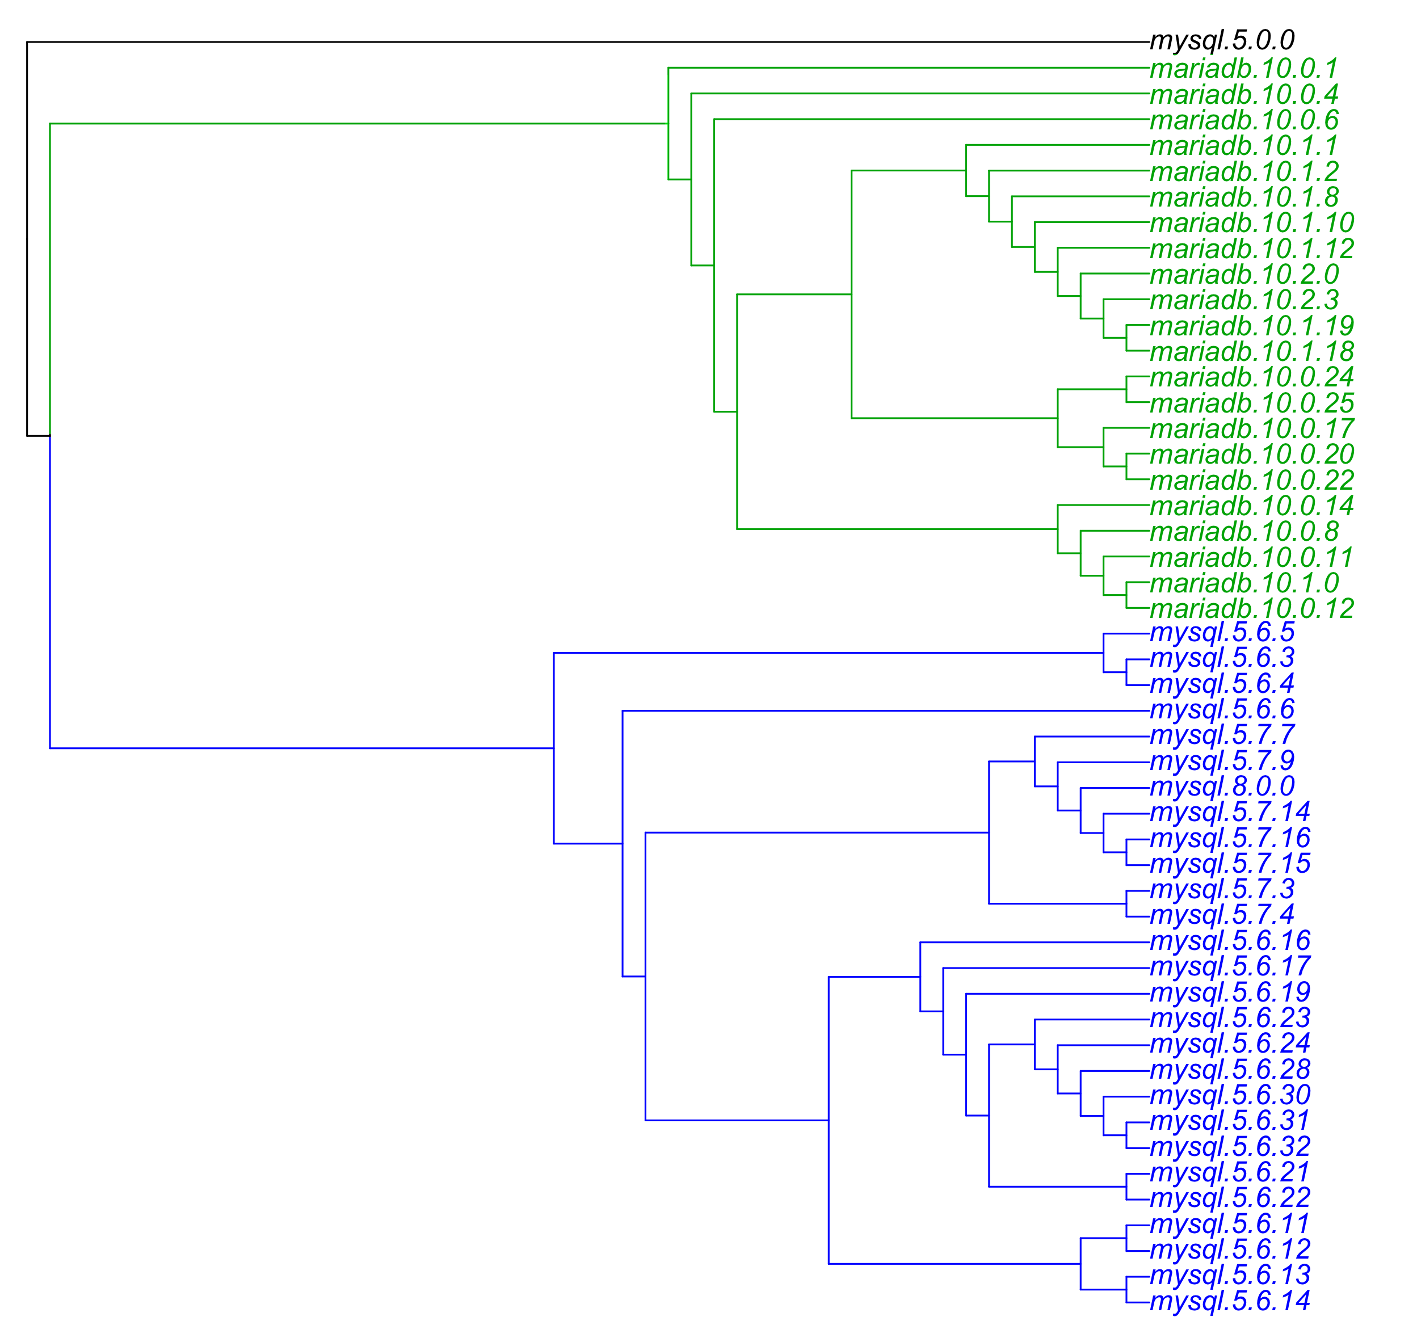
\includegraphics[width=\textwidth]{ext_tree.png}
  \caption{A phylogenetic tree of the MariaDB / MySQL fork.}
  \label{fig:ext_tree}
\end{figure}

%----------------------------------------------------------------------------------------

\section*{Key results}
Phylogenetic methods can, at least in the example shown above, provide a plausible reconstruction of the history of a fork. While this result is interesting as a proof-of-concept, it is not a key result, as a similar tree could have been obtained by examining the logs of the software repositories where the forked projects are kept. From a project management point of view, it is more interesting to know whether two parallel development strands are about to cross a threshold beyond which a fork will be unavoidable. As the analysis detailed in the next paragraph shows, it is possible to measure the pairwise dissimilarity between development branches within a project and therefore to detect those branches that have wandered the furthest from the main branch and could potentially fork.

Forks can have different outcomes. Forked projects may become each other's competitors, or the fork may result in the discontinuation of the original project. Alternatively, a project may fork yet the split teams may continue to exchange knowledge in a collaborative way. The second key result of the research is that the chosen measurements of intrinsic project properties are not sufficient to explain the outcome of a fork.

%----------------------------------------------------------------------------------------

\section*{Summary analysis}

Having constructed a phylogenetic tree, it becomes possible to measure the distance between the nodes of the tree. A statistical analysis of variance showed that, within each pair of forked projects examined, the mean pairwise distance between two releases on the same project is significantly smaller than the mean pairwise distance between releases on different projects, thus leading to the first key result.

If a fork results in competing projects, then different teams could be expected to produce different code bases. On the contrary, if the fork results in collaborating projects, different teams could be expected to produce code bases with many similarities. This idea was explored by constructing separate phylogenetic trees from measurements of (1) the code-base and of (2) the team data. A statistical analysis of variance did not find a significant correlation between the outcome of forks and the code-base- and team- measurements examined in this research, thus supporting the conclusion that other factors are responsible for the outcome of a fork.

%----------------------------------------------------------------------------------------

\section*{Summary discussion}

By constructing the phylogenetic tree of the forked projects and applying the analysis methods discussed above, it is possible to detect development strands that have wandered away from the main development branch, and therefore to estimate whether a development strand is likely to fork, even before the fork is effective. This is particularly interesting if forks are considered a risk.

On the other hand, the outcome of the forks used as examples for the research could not be related to the measurements obtained from the software's code base and team.

\section*{Key outcomes}

The selected case studies substantiate that well-known and large open source projects have been affected by forks and that major software companies have in some cases successfully used forks as a business strategy. Hence, forking is an important phenomenon in open source software development.

Methods for constructing phylogenetic trees, ported from evolutionary biology, proved useful for estimating the relationships between development strands. In particular, evidence was gained that forks can be predicted. Additionally, the research also suggests that managerial, economic, social or other socio-technical factors have a profound influence on the outcome of a fork.

Furthermore, the vocabulary used by evolutionary biologists to describe phylogenetic trees could be applicable for describing software evolution: in particular, the concepts of relatedness, clade, parsimony and convergent evolution seem be relevant to the history of software projects.

% ----------------------------------------------------------------------------------------
%	BIBLIOGRAPHY
%----------------------------------------------------------------------------------------

\bibliographystyle{abbrvnat}
\bibliography{master}

%----------------------------------------------------------------------------------------

\end{document}  

